\documentclass[a4paper, 12pt]{article}
\usepackage[utf8]{inputenc}
\renewcommand\familydefault{\sfdefault}
\usepackage[T1]{fontenc}
\usepackage[francais]{babel}
\usepackage[left=2.5cm,top=2.5cm,right=2.5cm,bottom=2.5cm]{geometry}
\usepackage{graphicx}
\usepackage[usenames, dvipsnames]{xcolor}
\definecolor{mygray}{gray}{0.95}

\usepackage{minted}
\usemintedstyle{colorful}
\usepackage{float}
\floatplacement{figure}{H}
\usepackage{authblk}
\usepackage{enumitem}
\usepackage{hyperref}
\hypersetup{
    colorlinks,
    citecolor=black,
    filecolor=black,
    linkcolor=black,
    urlcolor=blue
}

\usepackage{caption}
\newenvironment{code}{\captionsetup{type=listing}}{}
% \newenvironment{myminted}[bgcolor=mygray,breaklines,breaksymbol=,linenos,frame=single,stepnumber=1,tabsize=2]{text}
\usepackage{array}
\usepackage{etoolbox}
\patchcmd{\thebibliography}{\section*{\refname}}{}{}{}

\begin{document}

\title{BibApp Hepia}
\author{Steven Liatti}
\affil{\small Projet de semestre - Prof. Mickaël Hoerdt}
\affil{\small Hepia ITI 3\up{ème} année}
\maketitle

\begin{figure}
	\begin{center}
		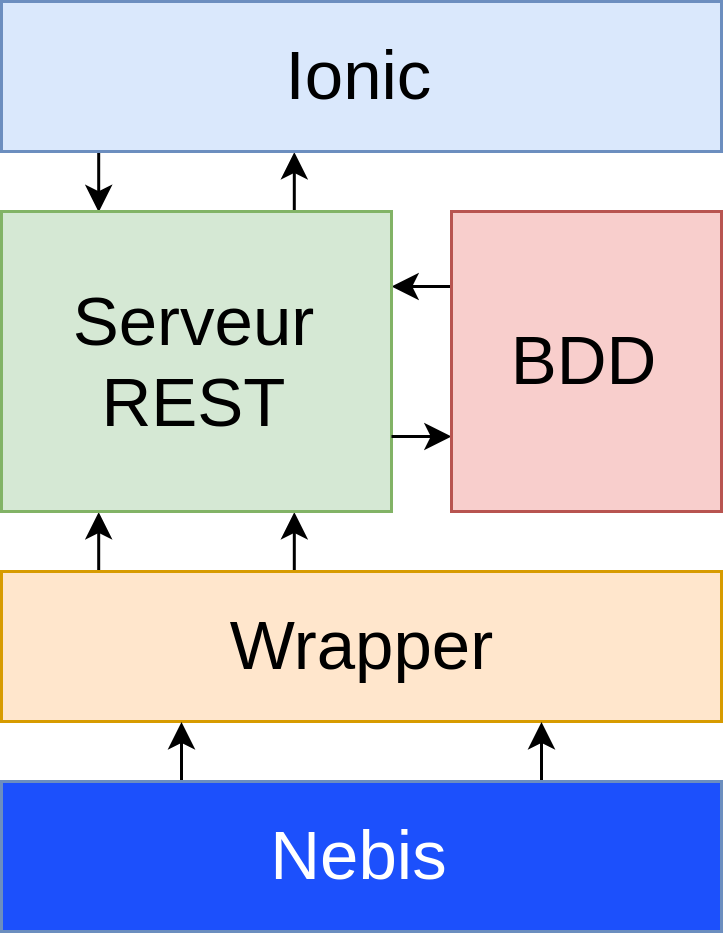
\includegraphics[width=0.5\textwidth]{images/architecture.png}
	\end{center}
\end{figure}

\begin{figure}[!b]
	\centering
	\begin{minipage}{.5\textwidth}
		\centering
		
\includegraphics[width=.7\linewidth]{images/hepia.jpg}
	\end{minipage}%
	\begin{minipage}{.5\textwidth}
		\centering
		
\includegraphics[width=.7\linewidth]{images/hesso.jpg}
	\end{minipage}
\end{figure}
\newpage

\newpage

\tableofcontents
\newpage
\listoffigures
\renewcommand\listoflistingscaption{Table des listings de code source}
\listoflistings
\newpage

\section{Introduction}
\subsection{BibApp V1}
\subsection{User stories}
\subsection{Besoins de la bibliothèque}
La bibliothèque de l'hepia aimerait attirer plus de monde en créant du contenu personnalisé autour de son
catalogue d'ouvrages et revues par le biais d'un site/application mobile. Voici les besoins listés plus
précisement :
\begin{itemize}
    \item Résumé d'un nouveau livre arrivé à la bibliothèque (nouveautés)
    \item Coups de coeur des bibliothécaires sur les ouvrages présents
    \item Revues de presse des périodiques
    \item Ajouter les images des couvertures scannées par la bibliothèque
\end{itemize}
Toutes ces actions doivent pouvoir être réalisées via le site web en mode administrateur. Les opérations de
création, récupération, modification et suppression de contenu (CRUD) sont nécessaires. Un mode utilisateur, ou visiteur,
permet de consulter le contenu, depuis un ordinateur ou un appareil mobile. L'idée est de créer une source
de contenus basée sur le catalogue Nebis et augmentée par les ajouts des bibliothécaires.

\section{Technologies utilisées}
\textit{Pour un aperçu rapide de Typescript et Angular, voir cet article de Josh Morony \cite{ref30}.}
\subsection{Typescript}
Ionic fait usage de \href{http://www.typescriptlang.org/}{Typescript}, une surcouche à Javascript, offrant des types
vérifés à la "compilation" (car Typescript est traduit, "transpiled", vers du Javascript conventionnel) et non à
l'exécution, signalant les erreurs sur les types et offrant ainsi plus de rigueur à l'écriture du code \cite{ref12}.

\begin{code}
    % \inputminted[bgcolor=mygray,breaklines,breaksymbol=,linenos,frame=single,stepnumber=1,tabsize=2]{language}{code}
    \begin{minted}[bgcolor=mygray,breaklines,breaksymbol=,linenos,frame=single,stepnumber=1,tabsize=2]{typescript}
function add(x : number, y : number) : number {
    return x + y;
}
add('a', 'b'); // compiler error

// Class example :
class Greeter {
    greeting: string;
    constructor (message: string) {
        this.greeting = message;
    }
    greet() {
        return "Hello, " + this.greeting;
    }
}
    \end{minted}
    \caption{Syntaxe Typescript}
    % \label{my_ref}
\end{code}
La structure basique des fichiers \textit{composants} Typescript avec Ionic ou Angular est semblable à ceci :
\begin{code}
    \begin{minted}[bgcolor=mygray,breaklines,breaksymbol=,linenos,frame=single,stepnumber=1,tabsize=2]{typescript}
import { Component } from '@angular/core';

@Component({
  selector: 'my-app'
})
export class AppComponent {
  title = 'My App';
  private field: string;

  constructor(public param: string) {
    this.field = param;
  }
}
    \end{minted}
    \caption{Exemple d'une classe Typescript sous Ionic ou Angular}
    % \label{my_ref}
\end{code}
Explications : on importe le composant \mintinline{typescript}{Component}, on définit le sélecteur utilisé dans le HTML
pour faire le rendu et on définit notre classe \mintinline{typescript}{AppComponent} qui pourra être exportée dans
d'autres modules. Dans cette classe nous définissons deux attributs \mintinline{typescript}{title} et
\mintinline{typescript}{field} et un constructeur. Typescript amène également une notion de visibilité des attributs 
et méthodes d'une classe, comme en Java.

\subsection{Angular 4}
\href{https://angular.io/}{Angular} \cite{ref15}, \cite{ref21} est un framework front-end Javascript développé par Google.
Je ne l'ai pas directement utilisé dans mon travail mais Ionic est construit sur Angular et partage de nombreux concepts
et fonctionnalités avec lui.
Angular impose une architecture de modules, où, pour chaque module, sont définis des fichiers HTML pour la structure
(avec une syntaxe ajoutée, voir plus loin), des fichiers CSS (ou autres préprocesseurs CSS comme
\href{http://sass-lang.com/}{Sass}) et des fichiers \textit{composant} écrits en Typescript, gérant la logique "métier".
\begin{figure}
    \begin{center}
        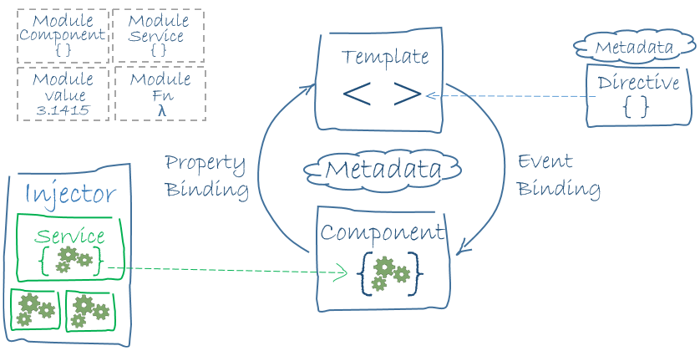
\includegraphics[width=0.8\textwidth]{images/angular2.png}
    \end{center}
    \caption{Architecture d'un composant Angular \cite{ref13}}
\end{figure}
Comme on peut apercevoir sur la figure ci-dessus, le template HTML intéragit avec son composant Typescript.
Un composant Angular est une simple classe Typescript, possédant attributs et méthodes.
Un template représente le combo page HTML et CSS, la vue du module, en interaction avec l'utilisateur.
Selon les actions de l'utilisateur, la vue ou le modèle (données) est mis à jour. On peut accéder aux attributs et méthodes
du composant depuis le template. Un ou plusieurs services peuvent être utilisés ("injectés") dans un module. On peut
voir un service comme un composant réutilisable et ne possédant pas (forcément) de template (exemples : services
d'authentification, de gestion d'images, etc.).
\bigbreak
Voici une brève description de balises et directives HTML ajoutées par Angular :
\begin{code}
    \begin{minted}[bgcolor=mygray,breaklines,breaksymbol=,linenos,frame=single,stepnumber=1,tabsize=2]{html}
<input [value]="firstName">
<button (click)="someFunction(event)">
<p>Hi, {{ name }} {{ 1 + 1 }}</p>
<input [(ngModel)]="name">
<p #myParagraph></p>
<section *ngIf="showSection">
<li *ngFor="let item of items">
    \end{minted}
    \caption{Syntaxe HTML avec Angular}
    % \label{my_ref}
\end{code}
Descriptif ligne par ligne :
\begin{enumerate}
    \item Change la propriété \mintinline{html}{value} en lui attribuant la vraie valeur de l'attribut de classe firstName (définit dans une classe Typescript)
    \item Appelle la fonction \mintinline{javascript}{someFunction()} en lui passant l'événement \mintinline{javascript}{event} au moment du clic sur le bouton
    \item Évalue les expressions entre {} et les affiche, ici en l'occurence un attribut \mintinline{javascript}{name} et le calcul de 1 + 1, 2
    \item Applique la valeur de \mintinline{javascript}{name} à l'input, mais s'il y a changement de la part de l'utilisateur, met à jour l'objet associé
    \item Crée une variable locale au template HTML
    \item \mintinline{html}{*ngIf} : supprime l'élément du DOM (ici \mintinline{html}{section}) si la condition n'est pas remplie
    \item \mintinline{html}{*ngFor} : boucle sur un tableau et répète l'élément du DOM
\end{enumerate}
\subsection{Ionic}
\subsection{Promise Javascript}
\subsection{Node.js}
\subsection{MongoDB}
\subsection{JSON Web Tokens}

\section{Tutoriel sur Ionic}
\textit{Ce tutoriel est réalisé avec la version 3.x.x de Ionic avec une machine sous Linux. Je me suis basé sur  
le tutoriel sur le site de Ionic \cite{ref0} et sur les tutoriels de Josh Morony \cite{ref10}, \cite{ref20}.}
\subsection{Installation}
Tout d'abord, Ionic nécessite Node.js et \mintinline{text}{npm}, son gestionnaire de paquets/dépendances Javascript. 
Une fois \mintinline{text}{npm} installé, il faut entrer la commande suivante dans un terminal :
\begin{code}
    \begin{minted}[bgcolor=mygray,breaklines,breaksymbol=,linenos,frame=single,stepnumber=1,tabsize=2]{bash}
npm install -g ionic cordova
    \end{minted}
    \caption{Installation de Ionic et Cordova}
    % \label{my_ref}
\end{code}
Cela installe Ionic et \href{https://cordova.apache.org}{Cordova}, l'outil permettant de traduire une web app à base de 
HTML, CSS et Javascript en application hybride (moitié native, moitié web) pour la plateforme choisie (Android, iOS, etc.). 
Pour créer un nouveau projet, il faut alors faire ceci :
\begin{code}
    \begin{minted}[bgcolor=mygray,breaklines,breaksymbol=,linenos,frame=single,stepnumber=1,tabsize=2]{bash}
ionic start myapp
cd myapp
ionic serve
    \end{minted}
    \caption{Initialisation d'un projet Ionic}
    % \label{my_ref}
\end{code}
La première commande crée l'arborescence de base d'un projet Ionic se nommant "myapp". Un menu interactif apparait avec 
plusieurs choix de template pour notre application : vide, avec des pages déjà intégrées ou un projet complet avec des pages 
et providers correspondant aux bonnes pratiques Ionic.
La dernière commande compile les sources Ionic dans le sous-dossier \mintinline{text}{www}
et lance un serveur web de développement en écoute sur \url{http://localhost:8100} qui compile à nouveau le projet à chaque 
changement dans le code.

\subsection{Ionic CLI}
Ionic fournit une interface en ligne de commande bien pratique. Elle permet de générer un projet avec choix de templates 
prédéfinis (\mintinline{bash}{ionic start}), de build l'application (\mintinline{bash}{ionic build}), de lancer l'application 
en mode développement avec \mintinline{bash}{ionic serve} et, commandes les plus pratiques, générer pages et providers entre 
autres (\mintinline{bash}{ionic g [page|provider] NewGenerate}). Un sous-ensemble de 
commandes avec le préfix \mintinline{bash}{ionic cordova} permet de build et lancer l'application Ionic sur des devices 
Android et iOS. Pour retrouver une aide sur toutes les commandes disponibles, entrez simplement \mintinline{bash}{ionic} 
dans un terminal.

\subsection{Arborescence}
Voici l'arborescence racine pour un projet Ionic, après avoir ajouté les plateformes désirées :
\begin{code}
    \begin{minted}[bgcolor=mygray,breaklines,breaksymbol=,linenos,frame=single,stepnumber=1,tabsize=2]{text}
.
|-- node_modules
|-- platforms
|-- plugins
|-- resources
|-- src
|-- www
|-- config.xml
|-- ionic.config.json
|-- package.json
|-- package-lock.json
|-- tsconfig.json
|-- tslint.json
    \end{minted}
    \caption{Arborescence racine}
    % \label{my_ref}
\end{code}
On peut apercevoir les dossier suivants : 
\begin{itemize}
    \item \mintinline{text}{node_modules} : contenant les dépendances Angular + Ionic
    \item \mintinline{text}{platforms} : contenant les builds et fichiers nécessaires des plateformes ajoutées avec cordova
    \item \mintinline{text}{plugins} : contenant les plugins Cordova
    \item \mintinline{text}{resources} : contenant les fichiers statiques pour Android et iOS (les icônes des applications notamment)
    \item \mintinline{text}{src} : contenant nos fichiers sources, c'est finalement le seul dossier qu'on utilise en développement
    \item \mintinline{text}{www} : contenant les fichiers construits ("build") à partir des sources, destinés à être servis par 
        un serveur web (tel qu'Apache)
\end{itemize}
Ensuite, le détail du dossier \mintinline{text}{src} : 
\\
\begin{code}
    \begin{minted}[bgcolor=mygray,breaklines,breaksymbol=,linenos,frame=single,stepnumber=1,tabsize=2]{text}
.
|-- app
│  |-- app.component.ts
│  |-- app.html
│  |-- app.module.ts
│  |-- app.scss
│  |-- main.ts
|-- assets
│  |-- icon
│  │  |-- favicon.ico
│  |-- imgs
│      |-- logo.png
|-- pages
│  |-- home
│      |-- home.html
│      |-- home.scss
│      |-- home.ts
|-- theme
│  |-- variables.scss
|-- index.html
|-- manifest.json
|-- service-worker.js
    \end{minted}
    \caption{Arborescence du dossier src}
    % \label{my_ref}
\end{code}
On peut apercevoir les dossier et fichiers suivants :
\begin{itemize}
    \item \mintinline{text}{app} : contient \mintinline{text}{app.component.ts} et \mintinline{text}{app.module.ts}, le composant principal et la liste des modules de l'application
    \item \mintinline{text}{assets} : les fichiers statiques tels que des images
    \item \mintinline{text}{pages} : contient toutes les pages générées avec Ionic CLI, c'est ici que s'écrit 90\% du code
    \item \mintinline{text}{theme} : contient \mintinline{text}{variable.scss}, un fichier sass avec les variables globales de l'application
\end{itemize}
\textit{Pour approfondir, je conseille de lire ce tutoriel \cite{ref20}.}

\subsection{Page}
Une page est constituée au minimum d'un fichier html (la vue) et Typescript (la logique métier). Pour personnaliser le 
design de la page uniquement, il est possible d'ajouter un fichier Sass (.scss) qui sera traduit en CSS. Chaque page doit être 
ajoutée au fichier \mintinline{text}{app.module.ts} pour pouvoir être importée et utilisée dans d'autres pages. Dans le fichier 
\mintinline{text}{app.component.ts} est définie la page principale (\mintinline{text}{root page}). Les pages se retrouvent 
par défaut dans le dossier \mintinline{text}{src/pages}. Par défaut, chaque page possède son propre dossier à son nom.

\subsection{Provider}
Un provider est un fournisseur de services aux pages de notre application. Il peut être vu comme une page sans vue, donc 
uniquement du Typescript, de la logique métier. Les providers servent généralement à fournir une API interne pour 
manipuler des données, qu'elles soient distantes ou locales. Il se retrouvent par défaut dans le dossier 
\mintinline{text}{src/providers}.

\subsection{Navigation}
Ionic utilise un système de pile pour la navigation entre ses pages. Selon si la page suivante a une relation 
semblable à celle "parent-enfant", ça vaut la peine de "push" la nouvelle page sur la première, pour facilement y 
revenir : par exemple, une liste d'articles, avec pour chaque article la possibilité de naviguer vers lui, il semble 
naturel de pouvoir facilement revenir à la liste des articles. Au contraire, si on change de section sur notre 
application ou si les deux pages n'ont pas de lien direct entre elles, il vaut mieux changer la \mintinline{text}{root page}, 
autrement dit, la "page racine". Une page parente a la possibilité de passer des paramètres à la page enfant. 
Tous ces mécanismes sont accessibles depuis le composant \mintinline{text}{NavController} \cite{ref50}.

\subsection{Composants disponibles}
Ionic fournit de nombreux composants graphiques  prêts à l'emploi pour l'interface utilisateur. La liste complète 
est disponible sur \url{https://ionicframework.com/docs/components/}. On y trouve par exemple des boutons prédéfinis 
mais personnalisables, des boutons flottants, des gestes (surtout pour le tactile), des listes, des modales, des menus,
une barre de recherche, des onglets, etc.

\subsection{Design}
Ionic offre des feuilles de style Sass et CSS préconçues. Une disposition des éléments 
selon une grille (à la manière de \href{http://getbootstrap.com/}{Bootstrap}) est disponible. Toutes les variables Sass 
sont modifiables dans le fichier \mintinline{text}{variables.scss}.

\subsection{Service HTTP}
Angular fournit un service HTTP, utilisable dans Ionic, pour faire des requêtes asynchrones. Exemple ici d'une 
requête \mintinline{text}{GET}. La fonction \mintinline{javascript}{map()} applique pour chaque élément des données 
reçues (un tableau par exemple) la fonction passée en argument et retourne un \mintinline{javascript}{Observable}. 
Ici on parse les données JSON reçues. Ensuite, dans \mintinline{javascript}{subscribe()}, trois cas de figure :
\begin{itemize}
    \item On accède aux données lorsqu'elles sont "prêtes"
    \item Si la requête a échoué, on affiche un message d'erreur (dans le cas présent)
    \item Enfin, on exécute les instructions dans tous les cas de figure
\end{itemize}
\begin{code}
    \begin{minted}[bgcolor=mygray,breaklines,breaksymbol=,linenos,frame=single,stepnumber=1,tabsize=2]{typescript}
this.http.get('http://example.com/api')
.map(res => res.json())
.subscribe(
  data => {
    // process data
  },
  err => {
    console.log("Error : ", err);
  },
  () => {
    // finally block
  }
);
    \end{minted}
    \caption{Requête HTTP avec Ionic}
    % \label{my_ref}
\end{code}

\subsection{Service Storage}
Ionic fournit une méthode simple pour stocker des données sour forme de paires clé/valeur sur le client local, 
que ce soit dans le navigateur ou dans l'application mobile. Une utilisation possible est de déclarer une classe 
qui fait appel à \mintinline{text}{storage} de la manière suivante \cite{ref70} :
\begin{code}
    \begin{minted}[bgcolor=mygray,breaklines,breaksymbol=,linenos,frame=single,stepnumber=1,tabsize=2]{typescript}
import { Storage } from '@ionic/storage';
import { Injectable } from '@angular/core';

@Injectable()
export class DataProvider {

  constructor(private storage: Storage) {}

  getPairs() {
    let pairs = [];
    this.storage.forEach((v, k) => {
      comments.push({key: k, value: v});
    });
    return pairs;
  }

  get(key: string) {
    return this.storage.get(key);
  }
 
  set(key: string, data: string) {
    this.storage.set(key, data);
  }

}
    \end{minted}
    \caption{Storage avec Ionic}
    % \label{my_ref}
\end{code}

\subsection{Déploiement}
Grâce une fois de plus à ls CLI Ionic, le déploiement d'une application Ionic est facilité. Pour plus d'informations, voir 
\href{https://ionicframework.com/docs/intro/deploying/}{cette page}.
\subsubsection{Browser}
Pour un déploiement à destination des navigateurs web, il faut se placer dans le dossier de l'application et, dans 
un terminal, entrer \mintinline{bash}{ionic build}. Ceci va compiler les fichiers Typescript, Sass et HTML dans le 
dossier \mintinline{text}{www}. Ce dossier peut ensuite facilement être ajouté à un serveur HTTP tel qu'Apache.

\subsubsection{Android}
Pour déployer sur un Android device, il faut au préalable avoir installé 
\href{http://www.oracle.com/technetwork/java/javase/downloads/index-jsp-138363.html}{Java JDK} et 
\href{https://developer.android.com/studio/index.html}{Android Studio} avec le SDK à jour. Il faut ensuite, dans un 
terminal, se positionner dans le dossier Ionic de l'application et lancer les commandes suivantes, pour build ou pour 
run l'application sur un device connecté : 
\begin{code}
    \begin{minted}[bgcolor=mygray,breaklines,breaksymbol=,linenos,frame=single,stepnumber=1,tabsize=2]{bash}
ionic cordova build android --device
# ou
ionic cordova run android --device
    \end{minted}
    \caption{Déploiement sur Android}
    % \label{my_ref}
\end{code}
\textbf{Astuce : } s'assurer que le path du SDK Android est bien configuré dans Cordova \cite{ref60}.

\subsubsection{iOS}
Bien que non testée, la procédure est similaire à Android. Il faut tout d'abord disposer d'un Mac avec Xcode 7 ou 
supérieur, un device avec iOS 9 ou plus et un \href{https://appleid.apple.com/}{Apple ID}. Ensuite dans un 
terminal, se positionner dans le dossier Ionic de l'application et lancer les commandes suivantes, pour build ou pour 
run l'application sur un device connecté : 
\begin{code}
    \begin{minted}[bgcolor=mygray,breaklines,breaksymbol=,linenos,frame=single,stepnumber=1,tabsize=2]{bash}
ionic cordova build ios --device
# ou
ionic cordova run ios --device
    \end{minted}
    \caption{Déploiement sur iOS}
    % \label{my_ref}
\end{code}

\section{Architecture}
Actuellement, le catalogue Nebis \cite{ref80} est utilisé par la bibliothèque. Cependant, il sera abandonné dans quelques
années pour un nouveau catalogue, encore inconnu à ce jour. L'objectif étant de réaliser une web app pérenne,
il faut pouvoir s'adapter à ce changement. Voici ci-dessous l'architecture globale de l'application :
\begin{figure}
    \begin{center}
        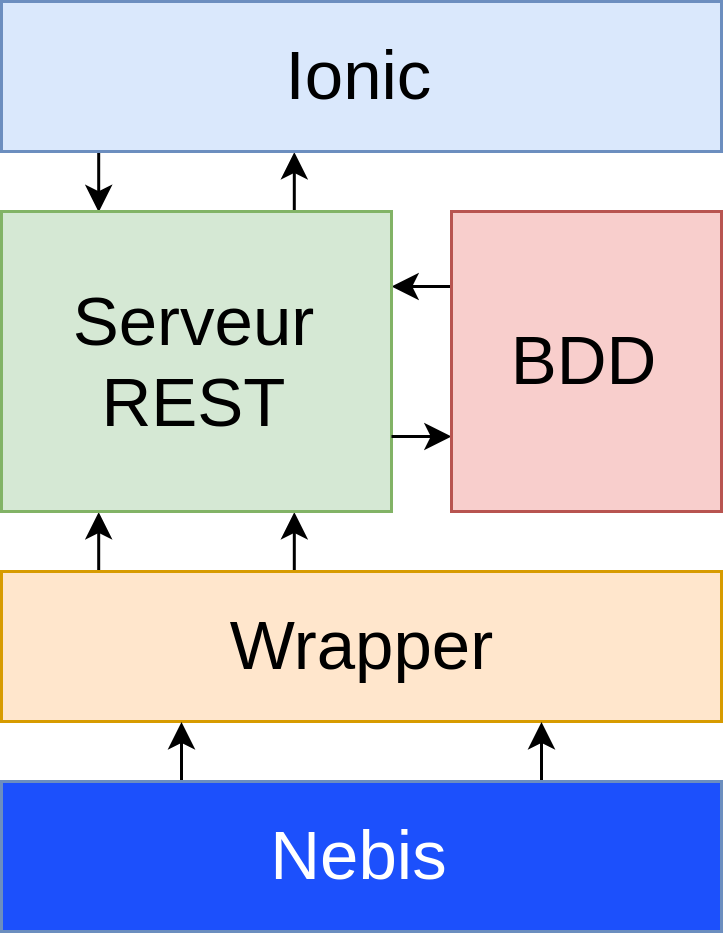
\includegraphics[width=0.5\textwidth]{images/architecture.png}
    \end{center}
    \caption{Architecture globale de la web app}
\end{figure}
Le Wrapper et le serveur REST seront faits en Node.js. La base de données sera faite avec MongoDB.

\subsection{Wrapper}
Ce module fait le pont entre les données issues d'un catalogue et le serveur REST. Son utilité principale est
de s'adapter au catalogue utilisé : si le catalogue est amené à changer ou à disparaître au profit d'un autre,
il suffira de modifier ce Wrapper pour continuer à faire fonctionner l'application. Il devra au minimum fournir :
\begin{itemize}
    \item La liste des nouveautés
    \item Les informations de base sur les ouvrages
    \item La recherche d'une oeuvre par ISBN et/ou d'autres critères
\end{itemize}


\subsection{Serveur REST}
Ce serveur offre les services suivants :
\begin{itemize}
    \item CRUD pour les infos de base des oeuvres (Nebis)
    \item CRUD pour les résumés/commentaires des livres
    \item CRUD pour les coups de coeur des bibliothécaires
    \item CRUD pour les revues de presse
    \item CRUD pour les images scannées par les bibliothécaires
    \item Authentification et autorisations des utilisateurs
\end{itemize}

\subsection{Base de données augmentée}
La base de données sera liée au serveur REST, elle enregistrera le contenu produit par la bibliothèque.
\begin{figure}
    \begin{center}
        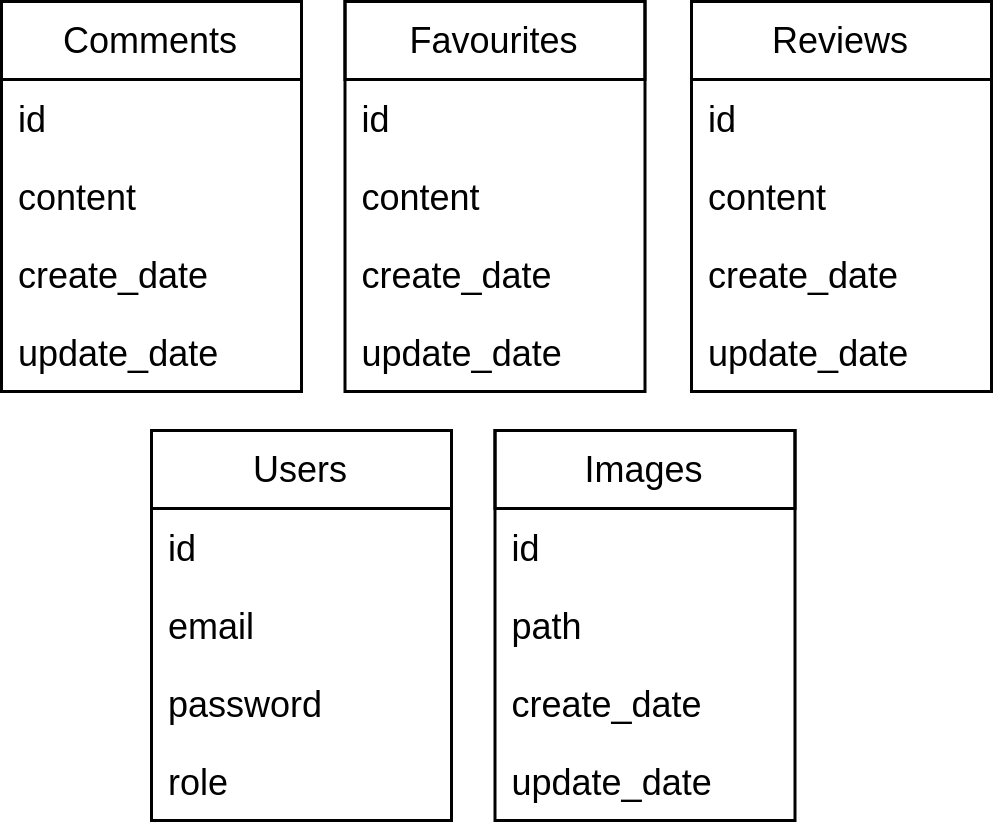
\includegraphics[width=0.9\textwidth]{images/bdd.png}
    \end{center}
    \caption{Schéma de la base de données}
\end{figure}
\textit{(Ce schéma est amené à évoluer)}

\subsection{Ionic}
Partie front-end de l'application, elle offrira côté utilisateur :
\begin{itemize}
    \item Page d'accueil, avec les sections "Nouveautés", "Coups de coeur" et "Revues de presse"
    \item Pour chaque section, une page listant les ouvrages ou périodiques avec infos de base
        (Titre, auteur, etc. et image si fournie)
    \item Pour chaque entrée, la possibilité de cliquer dessus et consulter les infos Nebis et le contenu enrichi
\end{itemize}
Côté administrateur (ou rédacteur), les bibliothécaires pourront s'authentifier et auront une section supplémentaire,
"Images", où ils pourront ajouter les scans des livres aux entrées existantes. Pour les autres sections, ils
pourront ajouter le contenu correspondant aux entrées voulues.


\section{Réalisation}
\subsection{Captures d'écran}
\section{Guide de déploiement}
\section{Conclusion}

\section{Annexes}

\section{Références}
\bibliographystyle{unsrt}
\bibliography{bib}

\end{document}
